\section{Inserção}

\begin{frame}[fragile]{Inserção no início}

    \begin{itemize}
        \item A inserção no início (\code{c++}{push_front()}) de uma lista encadeada tem
            complexidade $O(1)$

        \item O primeiro passo da inserção é criar um novo nó

        \item Em seguida, deve ser preenchido o campo \code{c++}{info}

        \item O membro \code{c++}{next} deve apontar então para o primeiro elemento da lista
        (\code{c++}{head})

        \item Por fim, o membro \code{c++}{head} deve apontar para o novo elemento

        \item \textit{Corner case:} caso o membro \code{c++}{head} esteja nulo no início da 
            inserção, o membro \code{c++}{tail} também deve apontar para o novo elemento

        \item Caso a classe tenha o membro \code{cpp}{size}, este deve ser incrementado
            na inserção
    \end{itemize}

\end{frame}

\begin{frame}[fragile]{Visualização da inserção no início}

    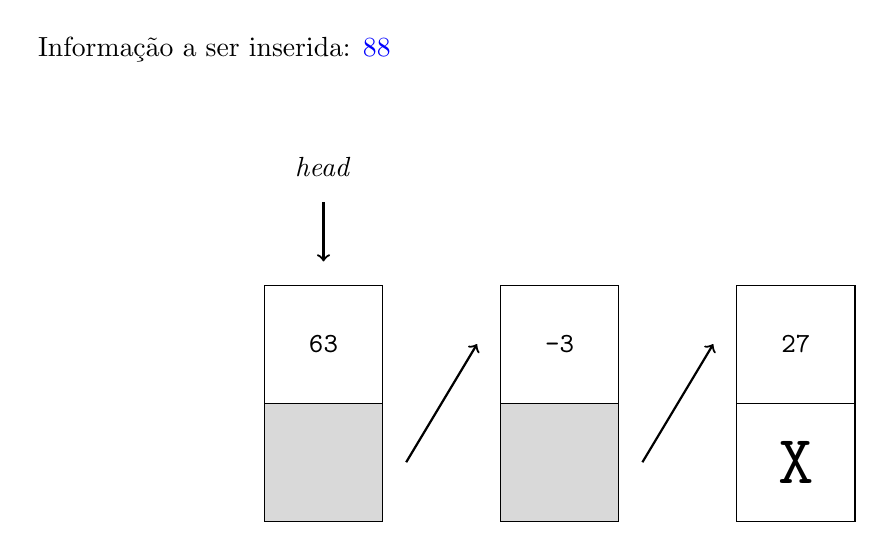
\begin{tikzpicture}[scale=1.5]
        \node[anchor=west] at (0, 4) {Informação a ser inserida: \textcolor{blue}{88}};

        \node[anchor=center] at (2.5, 3) {\textit{head}};
        \draw[->,thick] (2.5, 2.7) -- (2.5, 2.2);

        \draw[white] (0,1) rectangle (1,2);
%        \draw[fill=gray!30] (0,0) rectangle (1,1);
%        \node at (0.5,1.5) {\texttt{15}};

%        \draw[->,thick] (1.2, 0.5) -- (1.8, 1.5);
        \draw[fill=white] (2,1) rectangle (3,2);
        \draw[fill=gray!30] (2,0) rectangle (3,1);
        \node at (2.5,1.5) {\texttt{63}};

        \draw[->,thick] (3.2, 0.5) -- (3.8, 1.5);
        \draw[fill=white] (4,1) rectangle (5,2);
        \draw[fill=gray!30] (4,0) rectangle (5,1);
        \node at (4.5,1.5) {\texttt{-3}};

        \draw[->,thick] (5.2, 0.5) -- (5.8, 1.5);
        \draw[fill=white] (6,1) rectangle (7,2);
        \draw (6,0) rectangle (7,1);
        \node at (6.5,1.5) {\texttt{27}};
        \node at (6.5,0.5) {\Huge \textbf{\texttt{X}}};

    \end{tikzpicture}

\end{frame}

\begin{frame}[fragile]{Visualização da inserção no início}

    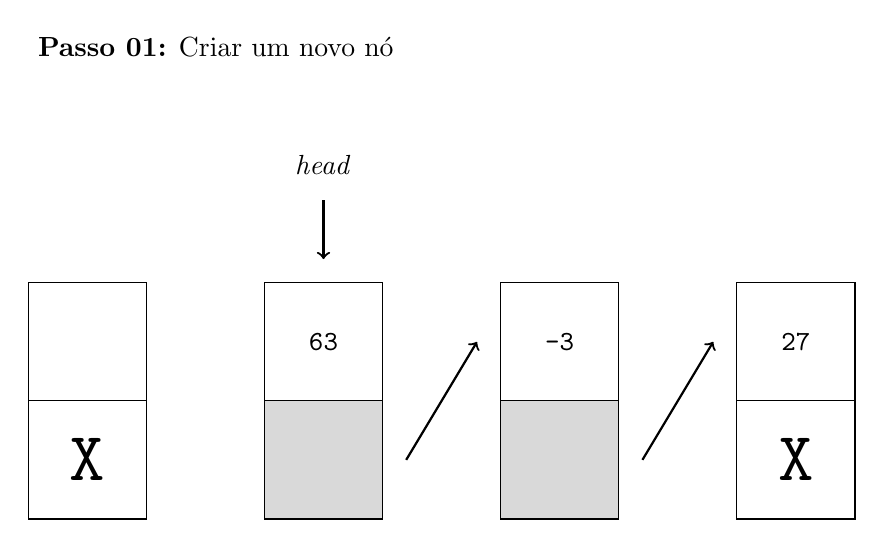
\begin{tikzpicture}[scale=1.5]
        \node[anchor=west] at (0, 4) {\textbf{Passo 01:} Criar um novo nó};

        \node[anchor=center] at (2.5, 3) {\textit{head}};
        \draw[->,thick] (2.5, 2.7) -- (2.5, 2.2);

        \draw (0,1) rectangle (1,2);
        \node at (0.5,0.5) {\Huge \textbf{\texttt{X}}};
        \draw (0,0) rectangle (1,1);
%        \node at (0.5,1.5) {\texttt{15}};

%        \draw[->,thick] (1.2, 0.5) -- (1.8, 1.5);
        \draw[fill=white] (2,1) rectangle (3,2);
        \draw[fill=gray!30] (2,0) rectangle (3,1);
        \node at (2.5,1.5) {\texttt{63}};

        \draw[->,thick] (3.2, 0.5) -- (3.8, 1.5);
        \draw[fill=white] (4,1) rectangle (5,2);
        \draw[fill=gray!30] (4,0) rectangle (5,1);
        \node at (4.5,1.5) {\texttt{-3}};

        \draw[->,thick] (5.2, 0.5) -- (5.8, 1.5);
        \draw[fill=white] (6,1) rectangle (7,2);
        \draw (6,0) rectangle (7,1);
        \node at (6.5,1.5) {\texttt{27}};
        \node at (6.5,0.5) {\Huge \textbf{\texttt{X}}};

    \end{tikzpicture}

\end{frame}

\begin{frame}[fragile]{Visualização da inserção no início}

    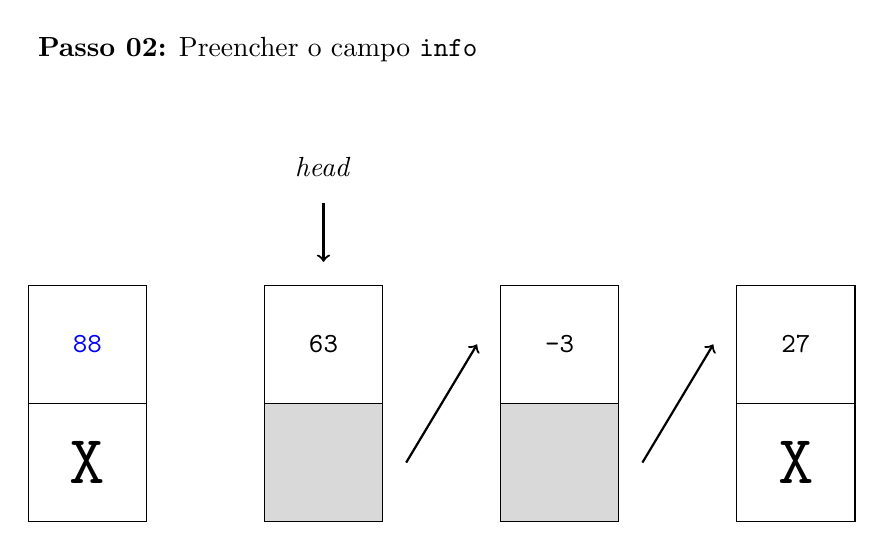
\begin{tikzpicture}[scale=1.5]
        \node[anchor=west] at (0, 4) {\textbf{Passo 02:} Preencher o campo \texttt{info}};

        \node[anchor=center] at (2.5, 3) {\textit{head}};
        \draw[->,thick] (2.5, 2.7) -- (2.5, 2.2);

        \draw (0,1) rectangle (1,2);
        \node at (0.5,0.5) {\Huge \textbf{\texttt{X}}};
        \draw (0,0) rectangle (1,1);
        \node at (0.5,1.5) {\texttt{\textcolor{blue}{88}}};

%        \draw[->,thick] (1.2, 0.5) -- (1.8, 1.5);
        \draw[fill=white] (2,1) rectangle (3,2);
        \draw[fill=gray!30] (2,0) rectangle (3,1);
        \node at (2.5,1.5) {\texttt{63}};

        \draw[->,thick] (3.2, 0.5) -- (3.8, 1.5);
        \draw[fill=white] (4,1) rectangle (5,2);
        \draw[fill=gray!30] (4,0) rectangle (5,1);
        \node at (4.5,1.5) {\texttt{-3}};

        \draw[->,thick] (5.2, 0.5) -- (5.8, 1.5);
        \draw[fill=white] (6,1) rectangle (7,2);
        \draw (6,0) rectangle (7,1);
        \node at (6.5,1.5) {\texttt{27}};
        \node at (6.5,0.5) {\Huge \textbf{\texttt{X}}};

    \end{tikzpicture}

\end{frame}

\begin{frame}[fragile]{Visualização da inserção no início}

    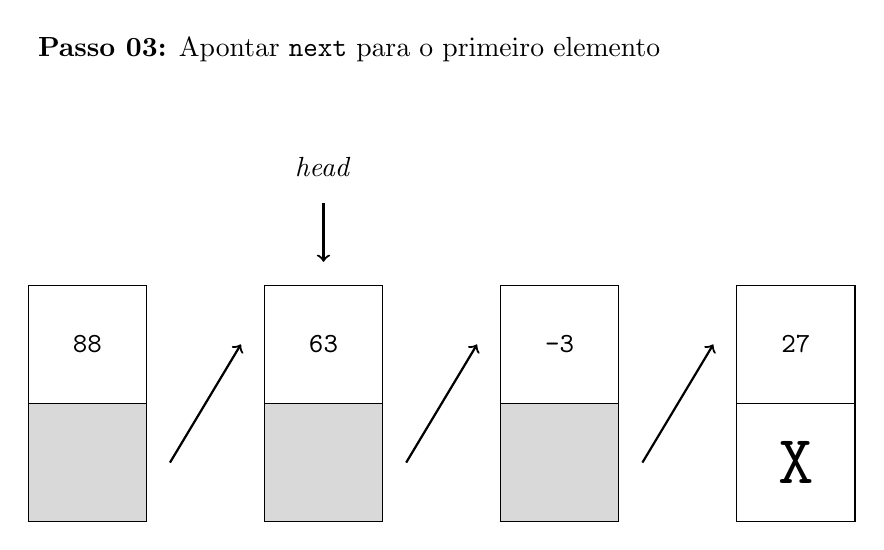
\begin{tikzpicture}[scale=1.5]
        \node[anchor=west] at (0, 4) {\textbf{Passo 03:} Apontar \texttt{next} para o primeiro elemento};

        \node[anchor=center] at (2.5, 3) {\textit{head}};
        \draw[->,thick] (2.5, 2.7) -- (2.5, 2.2);

        \draw (0,1) rectangle (1,2);
        \draw[fill=gray!30] (0,0) rectangle (1,1);
        \node at (0.5,1.5) {\texttt{\textcolor{black}{88}}};

        \draw[->,thick] (1.2, 0.5) -- (1.8, 1.5);
        \draw[fill=white] (2,1) rectangle (3,2);
        \draw[fill=gray!30] (2,0) rectangle (3,1);
        \node at (2.5,1.5) {\texttt{63}};

        \draw[->,thick] (3.2, 0.5) -- (3.8, 1.5);
        \draw[fill=white] (4,1) rectangle (5,2);
        \draw[fill=gray!30] (4,0) rectangle (5,1);
        \node at (4.5,1.5) {\texttt{-3}};

        \draw[->,thick] (5.2, 0.5) -- (5.8, 1.5);
        \draw[fill=white] (6,1) rectangle (7,2);
        \draw (6,0) rectangle (7,1);
        \node at (6.5,1.5) {\texttt{27}};
        \node at (6.5,0.5) {\Huge \textbf{\texttt{X}}};

    \end{tikzpicture}

\end{frame}

\begin{frame}[fragile]{Visualização da inserção no início}

    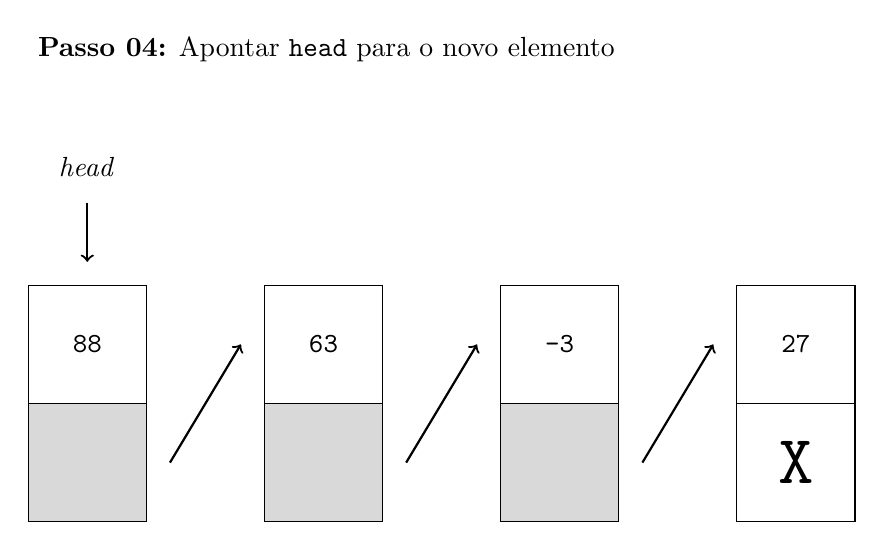
\begin{tikzpicture}[scale=1.5]
        \node[anchor=west] at (0, 4) {\textbf{Passo 04:} Apontar \texttt{head} para o novo elemento};

        \node[anchor=center] at (0.5, 3) {\textit{head}};
        \draw[->,thick] (0.5, 2.7) -- (0.5, 2.2);

        \draw (0,1) rectangle (1,2);
        \draw[fill=gray!30] (0,0) rectangle (1,1);
        \node at (0.5,1.5) {\texttt{\textcolor{black}{88}}};

        \draw[->,thick] (1.2, 0.5) -- (1.8, 1.5);
        \draw[fill=white] (2,1) rectangle (3,2);
        \draw[fill=gray!30] (2,0) rectangle (3,1);
        \node at (2.5,1.5) {\texttt{63}};

        \draw[->,thick] (3.2, 0.5) -- (3.8, 1.5);
        \draw[fill=white] (4,1) rectangle (5,2);
        \draw[fill=gray!30] (4,0) rectangle (5,1);
        \node at (4.5,1.5) {\texttt{-3}};

        \draw[->,thick] (5.2, 0.5) -- (5.8, 1.5);
        \draw[fill=white] (6,1) rectangle (7,2);
        \draw (6,0) rectangle (7,1);
        \node at (6.5,1.5) {\texttt{27}};
        \node at (6.5,0.5) {\Huge \textbf{\texttt{X}}};

    \end{tikzpicture}

\end{frame}

\begin{frame}[fragile]{Implementação da inserção no início}
    \inputsnippet{cpp}{41}{48}{list.h}
\end{frame}

\begin{frame}[fragile]{Inserção no final}

    \begin{itemize}
        \item A inserção no final (\code{c++}{push_back()}) de uma lista encadeada tem
            complexidade $O(1)$, desde que a classe tenha o membro \code{c++}{tail}

        \item O primeiro passo da inserção é criar um novo nó

        \item Em seguida, deve ser preenchido o campo \code{c++}{info}

        \item O membro \code{c++}{next} de \code{c++}{tail} deve apontar então para 
        o novo elemento da lista

        \item Por fim, o membro \code{c++}{tail} deve apontar para o novo elemento

        \item \textit{Corner case:} caso o membro \code{c++}{tail} esteja nulo no início da 
            inserção, o membro \code{c++}{head} também deve apontar para o novo elemento

        \item Caso a classe tenha o membro \code{cpp}{size}, este deve ser incrementado
            na inserção
    \end{itemize}

\end{frame}

\begin{frame}[fragile]{Visualização da inserção no final}

    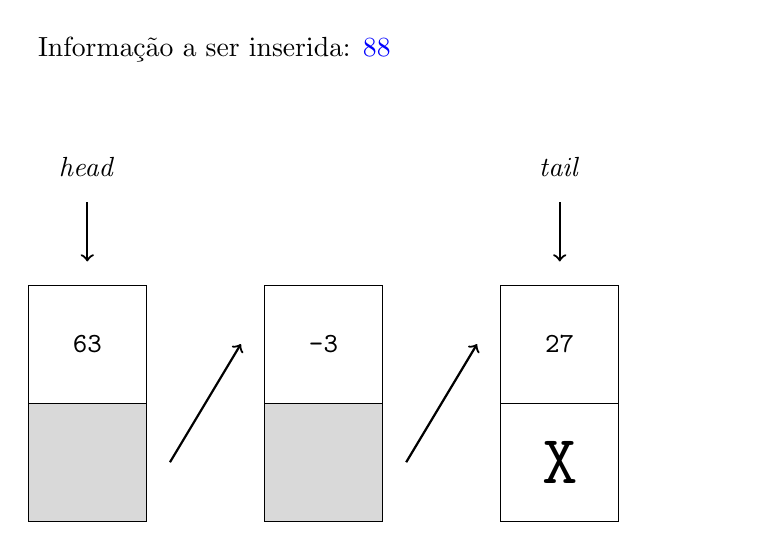
\begin{tikzpicture}[scale=1.5]
        \node[anchor=west] at (0, 4) {Informação a ser inserida: \textcolor{blue}{88}};

        \node[anchor=center] at (0.5, 3) {\textit{head}};
        \draw[->,thick] (0.5, 2.7) -- (0.5, 2.2);

        \node[anchor=center] at (4.5, 3) {\textit{tail}};
        \draw[->,thick] (4.5, 2.7) -- (4.5, 2.2);

        \draw[white] (6,1) rectangle (1,2);
%        \draw[fill=gray!30] (0,0) rectangle (1,1);
%        \node at (0.5,1.5) {\texttt{15}};

%        \draw[->,thick] (1.2, 0.5) -- (1.8, 1.5);
        \draw[fill=white] (0,1) rectangle (1,2);
        \draw[fill=gray!30] (0,0) rectangle (1,1);
        \node at (0.5,1.5) {\texttt{63}};

        \draw[->,thick] (1.2, 0.5) -- (1.8, 1.5);
        \draw[fill=white] (2,1) rectangle (3,2);
        \draw[fill=gray!30] (2,0) rectangle (3,1);
        \node at (2.5,1.5) {\texttt{-3}};

        \draw[->,thick] (3.2, 0.5) -- (3.8, 1.5);
        \draw[fill=white] (4,1) rectangle (5,2);
        \draw (4,0) rectangle (5,1);
        \node at (4.5,1.5) {\texttt{27}};
        \node at (4.5,0.5) {\Huge \textbf{\texttt{X}}};

    \end{tikzpicture}

\end{frame}

\begin{frame}[fragile]{Visualização da inserção no final}

    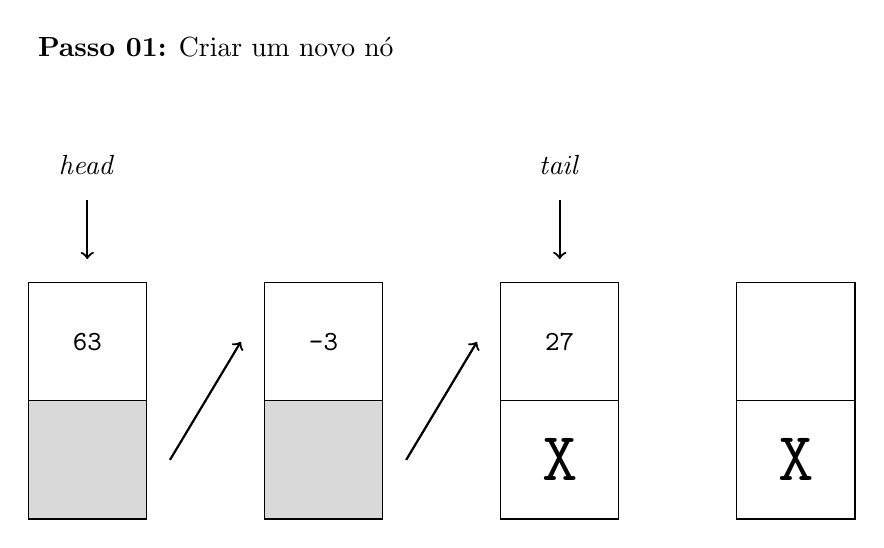
\begin{tikzpicture}[scale=1.5]
        \node[anchor=west] at (0, 4) {\textbf{Passo 01:} Criar um novo nó};

        \node[anchor=center] at (0.5, 3) {\textit{head}};
        \draw[->,thick] (0.5, 2.7) -- (0.5, 2.2);

        \node[anchor=center] at (4.5, 3) {\textit{tail}};
        \draw[->,thick] (4.5, 2.7) -- (4.5, 2.2);

        \draw (6,1) rectangle (7,2);
        \draw (6,0) rectangle (7,1);
        \node at (6.5,0.5) {\Huge \textbf{\texttt{X}}};
%        \node at (0.5,1.5) {\texttt{15}};

%        \draw[->,thick] (1.2, 0.5) -- (1.8, 1.5);
        \draw[fill=white] (0,1) rectangle (1,2);
        \draw[fill=gray!30] (0,0) rectangle (1,1);
        \node at (0.5,1.5) {\texttt{63}};

        \draw[->,thick] (1.2, 0.5) -- (1.8, 1.5);
        \draw[fill=white] (2,1) rectangle (3,2);
        \draw[fill=gray!30] (2,0) rectangle (3,1);
        \node at (2.5,1.5) {\texttt{-3}};

        \draw[->,thick] (3.2, 0.5) -- (3.8, 1.5);
        \draw[fill=white] (4,1) rectangle (5,2);
        \draw (4,0) rectangle (5,1);
        \node at (4.5,1.5) {\texttt{27}};
        \node at (4.5,0.5) {\Huge \textbf{\texttt{X}}};

    \end{tikzpicture}

\end{frame}

\begin{frame}[fragile]{Visualização da inserção no final}

    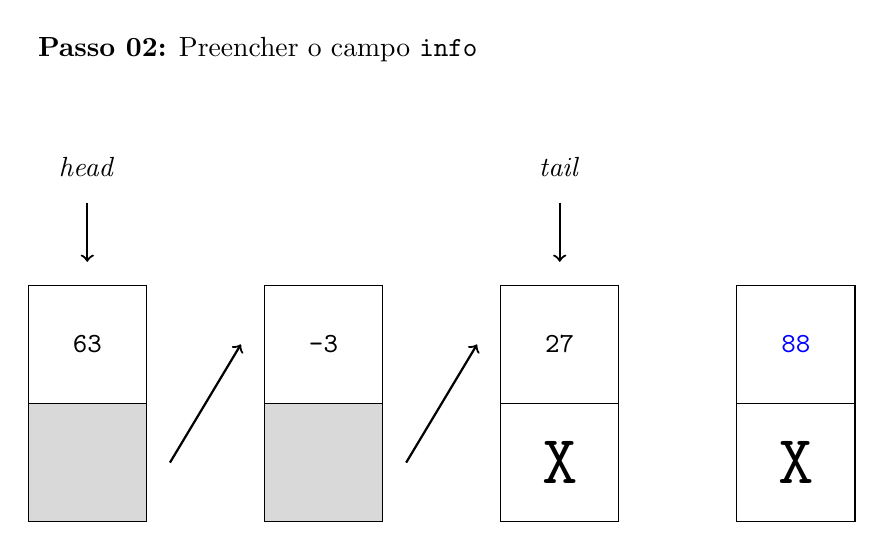
\begin{tikzpicture}[scale=1.5]
        \node[anchor=west] at (0, 4) {\textbf{Passo 02:} Preencher o campo \texttt{info}};

        \node[anchor=center] at (0.5, 3) {\textit{head}};
        \draw[->,thick] (0.5, 2.7) -- (0.5, 2.2);

        \node[anchor=center] at (4.5, 3) {\textit{tail}};
        \draw[->,thick] (4.5, 2.7) -- (4.5, 2.2);

        \draw (6,1) rectangle (7,2);
        \draw (6,0) rectangle (7,1);
        \node at (6.5,0.5) {\Huge \textbf{\texttt{X}}};
        \node at (6.5,1.5) {\texttt{\textcolor{blue}{88}}};

%        \draw[->,thick] (1.2, 0.5) -- (1.8, 1.5);
        \draw[fill=white] (0,1) rectangle (1,2);
        \draw[fill=gray!30] (0,0) rectangle (1,1);
        \node at (0.5,1.5) {\texttt{63}};

        \draw[->,thick] (1.2, 0.5) -- (1.8, 1.5);
        \draw[fill=white] (2,1) rectangle (3,2);
        \draw[fill=gray!30] (2,0) rectangle (3,1);
        \node at (2.5,1.5) {\texttt{-3}};

        \draw[->,thick] (3.2, 0.5) -- (3.8, 1.5);
        \draw[fill=white] (4,1) rectangle (5,2);
        \draw (4,0) rectangle (5,1);
        \node at (4.5,1.5) {\texttt{27}};
        \node at (4.5,0.5) {\Huge \textbf{\texttt{X}}};

    \end{tikzpicture}

\end{frame}

\begin{frame}[fragile]{Visualização da inserção no final}

    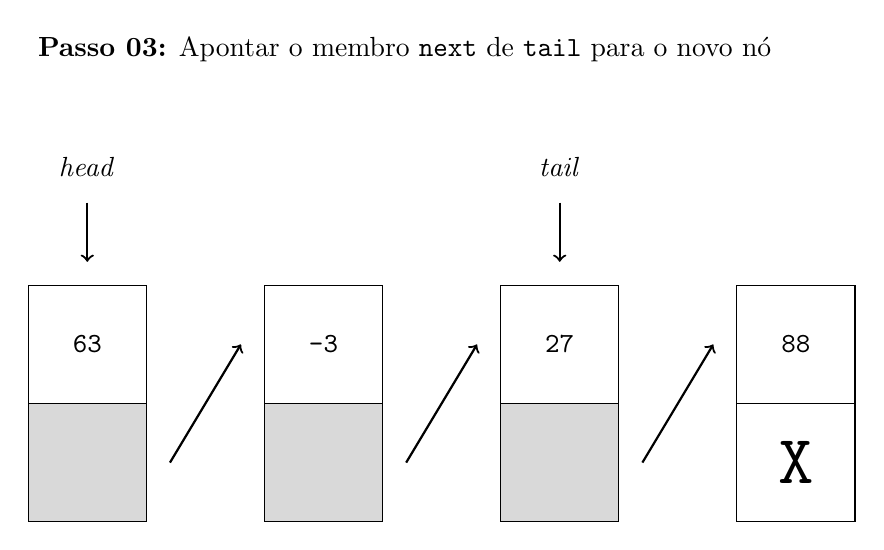
\begin{tikzpicture}[scale=1.5]
        \node[anchor=west] at (0, 4) {\textbf{Passo 03:} Apontar o membro \texttt{next} de \texttt{tail} para o novo nó};

        \node[anchor=center] at (0.5, 3) {\textit{head}};
        \draw[->,thick] (0.5, 2.7) -- (0.5, 2.2);

        \node[anchor=center] at (4.5, 3) {\textit{tail}};
        \draw[->,thick] (4.5, 2.7) -- (4.5, 2.2);

        \draw (6,1) rectangle (7,2);
        \draw (6,0) rectangle (7,1);
        \node at (6.5,0.5) {\Huge \textbf{\texttt{X}}};
        \node at (6.5,1.5) {\texttt{\textcolor{black}{88}}};

        \draw[->,thick] (5.2, 0.5) -- (5.8, 1.5);
        \draw[fill=white] (0,1) rectangle (1,2);
        \draw[fill=gray!30] (0,0) rectangle (1,1);
        \node at (0.5,1.5) {\texttt{63}};

        \draw[->,thick] (1.2, 0.5) -- (1.8, 1.5);
        \draw[fill=white] (2,1) rectangle (3,2);
        \draw[fill=gray!30] (2,0) rectangle (3,1);
        \node at (2.5,1.5) {\texttt{-3}};

        \draw[->,thick] (3.2, 0.5) -- (3.8, 1.5);
        \draw[fill=white] (4,1) rectangle (5,2);
        \draw[fill=gray!30] (4,0) rectangle (5,1);
        \node at (4.5,1.5) {\texttt{27}};

    \end{tikzpicture}

\end{frame}

\begin{frame}[fragile]{Visualização da inserção no final}

    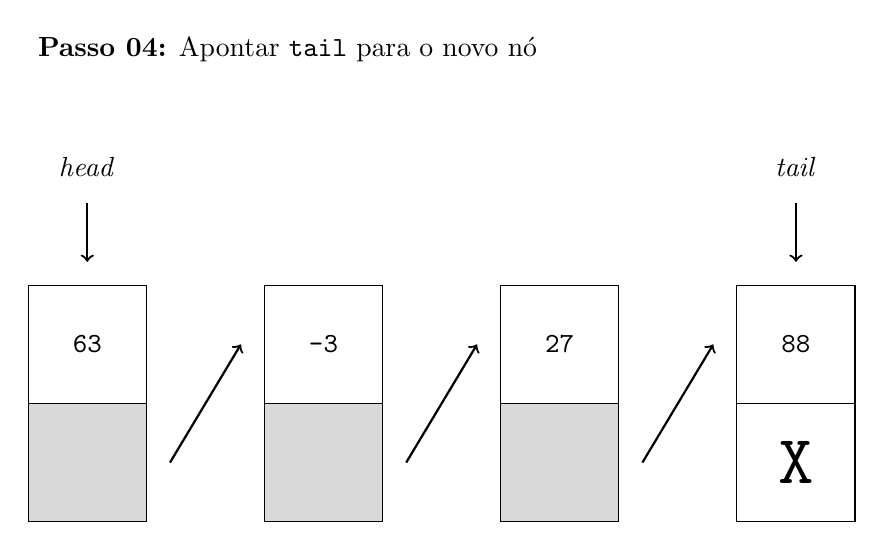
\begin{tikzpicture}[scale=1.5]
        \node[anchor=west] at (0, 4) {\textbf{Passo 04:} Apontar \texttt{tail} para o novo nó};

        \node[anchor=center] at (0.5, 3) {\textit{head}};
        \draw[->,thick] (0.5, 2.7) -- (0.5, 2.2);

        \node[anchor=center] at (6.5, 3) {\textit{tail}};
        \draw[->,thick] (6.5, 2.7) -- (6.5, 2.2);

        \draw (6,1) rectangle (7,2);
        \draw (6,0) rectangle (7,1);
        \node at (6.5,0.5) {\Huge \textbf{\texttt{X}}};
        \node at (6.5,1.5) {\texttt{\textcolor{black}{88}}};

        \draw[->,thick] (5.2, 0.5) -- (5.8, 1.5);
        \draw[fill=white] (0,1) rectangle (1,2);
        \draw[fill=gray!30] (0,0) rectangle (1,1);
        \node at (0.5,1.5) {\texttt{63}};

        \draw[->,thick] (1.2, 0.5) -- (1.8, 1.5);
        \draw[fill=white] (2,1) rectangle (3,2);
        \draw[fill=gray!30] (2,0) rectangle (3,1);
        \node at (2.5,1.5) {\texttt{-3}};

        \draw[->,thick] (3.2, 0.5) -- (3.8, 1.5);
        \draw[fill=white] (4,1) rectangle (5,2);
        \draw[fill=gray!30] (4,0) rectangle (5,1);
        \node at (4.5,1.5) {\texttt{27}};

    \end{tikzpicture}

\end{frame}

\begin{frame}[fragile]{Implementação da inserção no final}
    \inputsnippet{c++}{50}{57}{list.h}
\end{frame}

\begin{frame}[fragile]{Inserção em posição arbitrária}

    \begin{itemize}
        \item A inserção em posição arbitrária tem complexidade $O(N)$, onde $N$ é o número
            de elementos da lista 

        \item Primeiramente é necessário localizar a posição da inserção

        \item Além disso, é preciso identificar, se existir, o elemento que sucede o elemento que
            ocupa a posição de inserção

        \item O membro \code{c++}{next} do novo elemento deve apontar para o elemento que
            ocupa a posição de inserção

        \item O membro \code{c++}{next} do nó que antecedia o elemento da posição de inserção
            deve apontar para o novo nó

        \item É preciso tomar cuidado com vários \textit{corner cases}:
            \begin{enumerate}
                \item Lista vazia
                \item Apenas um elemento na lista
                \item Inserção na primeira posição
                \item Posição solicitada inválida
            \end{enumerate}

    \end{itemize}

\end{frame}
